\section{Forecasts}

\subsection{Optimising Design Variables}
In a world where time and money are both finite, it is essential that we plan our experiments carefully and know what results we can expect from them. Since PMF detection is not the primary goal of future CMB experiments, it is useful to know before carrying out the analysis whether they have a chance to detect PMFs. Additionally, if the case ever arises that an experiment is designed for the sole purpose of detecting the signatures of PMFs in the CMB, we'd like to know how best to design that experiment. The experiments I carried out this analysis for are stage-3 CMB experiments, such as SPT-3G or The Simons Array which will enter operation between 2016 and 2017. I also carried out this analysis for experiments similar to stage-4 CMB experiments, which are still in the planning stage.

\begin{figure}[h]
\centering
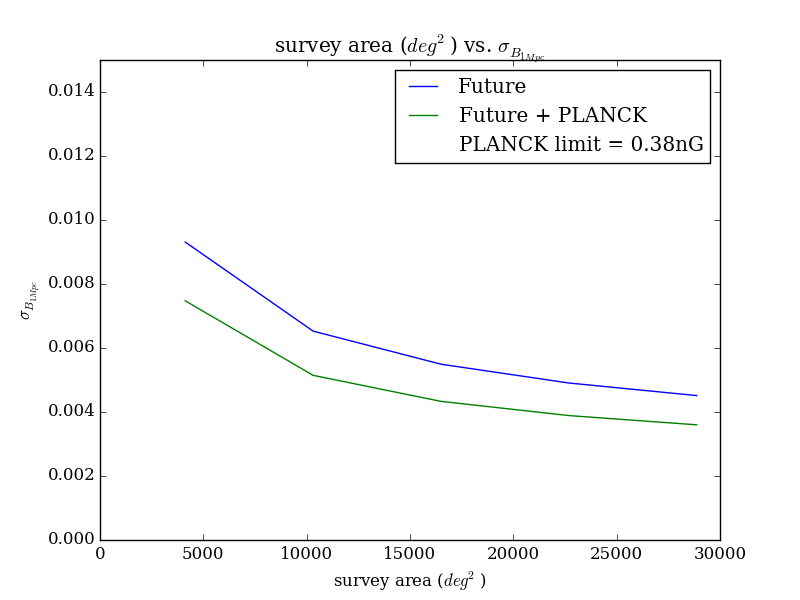
\includegraphics[scale=0.7]{images/area.png}
\caption{Increasing the survey area of future CMB experiments will return the best constraints on the value of $B_{1Mpc}$. This is a plot of survey area vs the uncertainty on $B_{1Mpc}$ with all other independent experimental variables held fixed. The blue line shows the precision for Future CMB experiments on their own and the green line shows the same precisions when combined with the PLANCK data set. Increasing survey area from 4125 deg$^2$ to 28877 deg$^2$ yields an improvement by roughly a factor of two. The best constraint is $\sigma(B_{1Mpc}) = 0.38nG$. Stage-3 and stage-4 will make a dramatic improvement over current PLANCK constraints of $\sigma(B_{1Mpc}) = 0.38nG$.}
\label{fig:area}
\end{figure}

\begin{figure}[h]
\centering
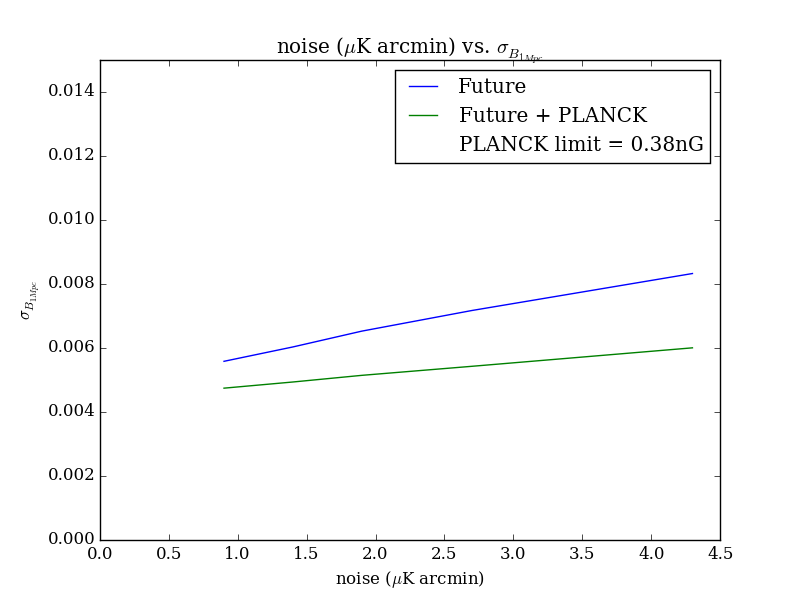
\includegraphics[scale=0.7]{images/noise.png}
\caption{Reducing the noise, which is done by adding more detectors to future CMB experiments constrains $B_{1Mpc}$ better than fewer detectors. This is a plot of noise vs the predicted uncertainty on $B_{1Mpc}$. The blue line shows the predicted limits on $\sigma(B_{1Mpc})$ from future CMB experiments and the green line shows the predicted limits on $\sigma(B_{1Mpc})$ for future experiments combined with current PLANCK constraints. The minimum noise of 0.9$\mu$K arcmin corresponds with a detector count of $\sim$500 000 detectors. At this noise level $\sigma(B_{1Mpc}) \geq 0.0048nG$. This is a significant increase in precision over the current PLANCK limit, $\sigma(B_{1Mpc}) = 0.38nG$.}
\label{fig:noise}
\end{figure}

\begin{figure}[h]
\centering
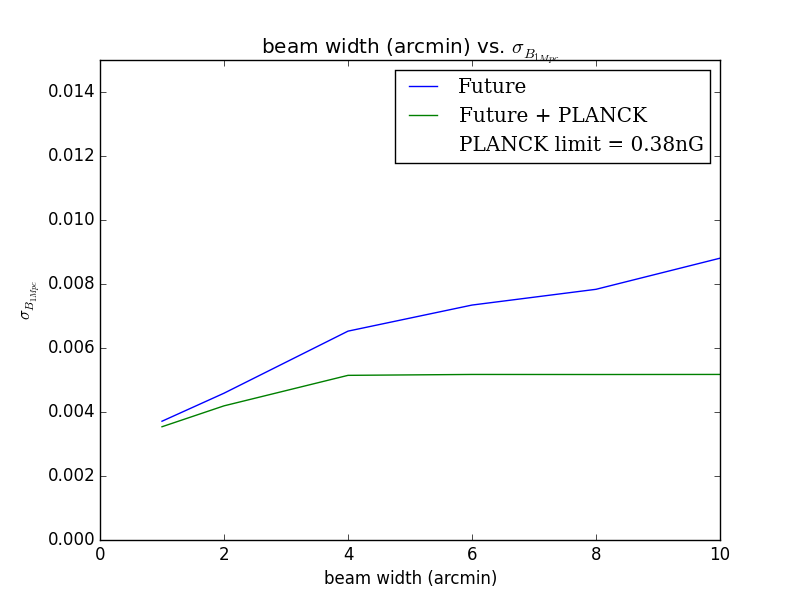
\includegraphics[scale=0.7]{images/width.png}
\caption{Reducing the the width of the beam, achieved by increasing the size of the telescope, reduces $\sigma(B_{1Mpc})$. This is a plot of beam width vs the uncertainty on $B_{1Mpc}$. The blue line shows the best constraints for $B_{1Mpc}$ for future CMB experiments and the green like shows the best constraints for $B_{1Mpc}$ for future CMB experiments plus PLANCK's constraints. The peak sensitivity for a beam width of 1 arcmin is $\sigma(B_{1Mpc}) \geq 0.0035nG$. This constraint is a major improvement over current PLANCK limits of $\sigma(B_{1Mpc}) = 0.38nG$.}
\label{fig:width}
\end{figure}

\begin{figure}[h]
\centering
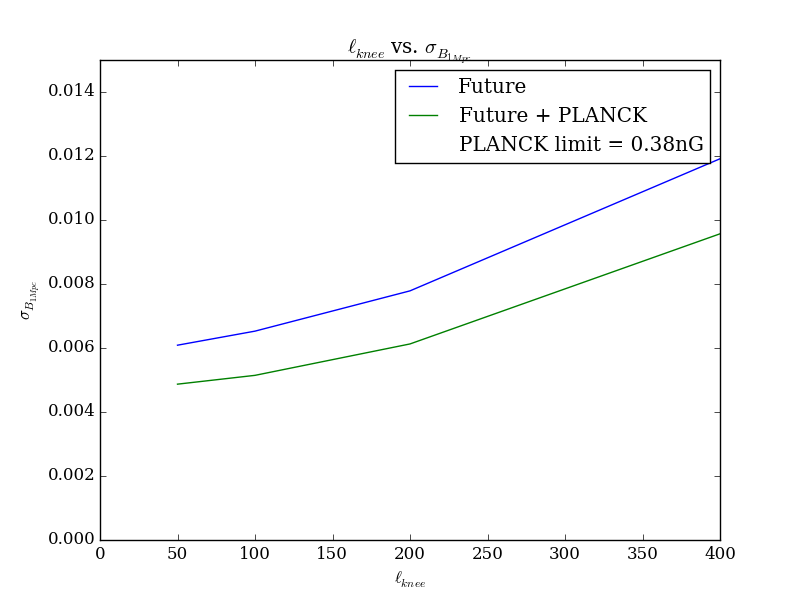
\includegraphics[scale=0.7]{images/knee.png}
\caption{Reducing $\ell_{knee}$ and hence increasing the stability of the experiment, also reduces $\sigma(B_{1Mpc})$. This is a plot of uncertainty on $B_{1Mpc}$ with all other variables held fixed. The blue line shows the best possible $\sigma(B_{1Mpc})$ for future experiments and the green line shows the best constraints for $\sigma(B_{1Mpc})$ for future experiments combined with prior limits from PLANCK. stage-3 and stage-4 shows a vast improvement over PLANCK's present limit of $\sigma(B_{1Mpc}) = 0.38nG$}
\label{fig:knee}
\end{figure}


In order to find the best experimental set up and quanitify the improvement from current levels to stage-3 or stage-4, I used the mock covariances as described in section 3.3. I looked at 6 different experimental variables: Survey area, detector noise, beam width, $\ell_{knee}$, beam uncertainty and calibration uncertainty. For a full description of these variables refer to section 3.3. By varying one experimental variable at a time and holding the rest fixed, I was able to forecast the minimum experimental uncertainty on the PMF strength, $\sigma(B_{1Mpc})$ for each mock experiment and plot the relationship between $\sigma(B_{1Mpc})$ and the experimental variables.

Table ~\ref{table: fixed-stats} shows the values I chose when I held an experimental variable fixed. The variables I chose represent an experiment somewhere between stage-3 and stage-4. The survey area is 10313 square degrees, which is typical for stage-3 experiment's survey area. On the other hand, the noise lies between a typical stage-3 and stage-4 experiment, at 1.9$\mu$K arcmin corresponding to a detector count of $\sim$50 000. I set $\ell_{knee} = 100$, corresponding to the standard for stage-3 and adopted a beam width of 4 arcmin, in line with both stage-3 and stage-4 values. Calibration error and beam uncertainty are set to 0.01$%$ and 0.05$%$ respectively, also matching both stage-3 and stage-4 specifications.

In Stage-3, we can expect $\sim$10 000 detectors. As a result the fixed value overestimates the noise reduction in stage-3. This means that the limits on $\sigma(B_{1Mpc})$ from stage-3 presented in this section will be smaller than the true value. On the other hand, since stage-4 will have a larger survey area, lower noise level and lower $\ell_{knee}$ (see Table ~\ref{table: stage-stats} for values), the limits on $\sigma(B_{1Mpc})$ will be severely underestimated. Stage-4 can do much better than the constraints shown here. Therefore it is best to consider the results in this section to be representative of a late-term stage-3 experiment rather than stage-4.

The optimal experimental design for detecting PMFs maximises the survey area and minimises the beam width, noise and $\ell_{knee}$. The sensitivity is independent of the beam and calibration uncertainties. As shown in figure ~\ref{fig:area}, $\sigma(B_{1Mpc})$ decreases as the survey area increases. If we combine the mock covariances with PLANCK data our best constraints range from $\sigma(B_{1Mpc}) \geq 0.0075nG$ for a survey area of 4125 deg$^2$ to $\sigma(B_{1Mpc}) \geq 0.0036nG$ for a survey area of 28877 deg$^2$, improving by a factor of 2.08. We also see a factor of 1.28 improvement, when the noise decreases from 4.3 $\mu$K arcmin to 0.9 $\mu$K arcmin, yielding  $\sigma(B_{1Mpc}) \geq 0.0060nG$ and $\sigma(B_{1Mpc}) \geq 0.0048nG$ respectively, as seen in figure ~\ref{fig:noise}. Decreasing the beam width from 10 arcmin to 1 arcmin improves sensitivity by a factor of 1.46 by reducing the uncertainty from $\sigma(B_{1Mpc}) \geq 0.0052nG$ to $\sigma(B_{1Mpc}) \geq 0.0035nG$ as per figure ~\ref{fig:width}. In figure ~\ref{fig:knee}, we see that a lower $\ell_{knee}$ improves sensitivity. At $\ell_{knee} = 50$, $\sigma(B_{1Mpc}) \geq 0.0049nG$ and in the worst-case scenario, when $\ell_{knee} = 400$, we have $\sigma(B_{1Mpc}) \geq 0.0096nG$ - a factor of 1.96 improvement. In contrast, changes to calibration and beam uncertainty have negligible effects on improving detection limits. For all values of beam and calibration uncertainties the sensitivity to the PMF strength is $\sigma(B_{1Mpc}) \geq 0.0051nG$.

The forecasts for the next stages of CMB experiments are promising. Our current best limits from Planck are $\sigma(B_{1Mpc}) = 0.38nG$. In comparison, the lowest limit from stage-3 and stage-4-like covariances are as low as $\sigma(B_{1Mpc}) = 0.0035nG$. In the most optimistic cases, measurements will have 100 times more sensitivity to PMFs than current experiments.

In practice, designing an experiment that satisfies all of these criteria for the minimum constraint on $B_{1Mpc}$ is incredibly difficult. Firstly, there's a tradeoff between noise and area. While adding detectors does reduce noise, so does time spent scanning per pixel - this is the depth. If we only have finite time on a telescope, we need to choose between a larger survey at a shallower depth or a smaller survey at a greater depth. Comparing figures, ~\ref{fig:area} and ~\ref{fig:noise} we see that larger survey areas generally produce better constraints on $B_{1Mpc}$ than lower noise. Therefore it seems reasonable that an experiment might prefer large survey areas over larger integration times.

A further problem with increasing the survey area is the galactic plane. The Milky Way galaxy blocks out light coming from the CMB and is a huge source of interference. As a result most experiments don't observe the full sky or at least cut it out of their maps, trading away survey area for clearer signals.

Another tradeoff is the beam width. Beam width is limited by how large we can build a telescope. If the telescope is too large, it becomes more expensive to build and maintain. In addition large telescopes become cumbersome and we may have to trade away some of our survey area to gain narrower beams. $\ell_{knee}$ is a technical constraint. Ideally we'd like to have $\ell_{knee} = 0$ of course in practice this simply won't happen since we can never reduce noise to zero. The tradeoff here is between money and quality. A device with a low $\ell_{knee}$ will likely be expensive and a device with a high $\ell_{knee}$ will be cheaper.  

\begin{table}[h]
\centering
\caption{Fixed Variables}
\label{table: fixed-stats}
\begin{tabular}{l|l}
\multicolumn{1}{c}{Variable} & \multicolumn{1}{|c}{Value} \\ \hline
\multicolumn{1}{c}{Survey area $(deg^2)$} & \multicolumn{1}{|c}{10313}  \\
\multicolumn{1}{c}{Noise ($\mu$K arcmin)} & \multicolumn{1}{|c}{1.9}   \\
\multicolumn{1}{c}{$\ell_{knee}$} & \multicolumn{1}{|c}{100} \\
\multicolumn{1}{c}{beam width (arcmin)} & \multicolumn{1}{|c}{4.0}   \\
\multicolumn{1}{c}{calibration error (\% error)} & \multicolumn{1}{|c}{0.01} \\
\multicolumn{1}{c}{beam uncertainty (\% error)} & \multicolumn{1}{|c}{0.05}
\end{tabular}
\begin{flushleft}
This table shows the values I chose for each independent variable when they were held fixed. The variables shown are all generous estimates for the range of capabilities the stage-3 experiments will have, but very conservative for stage-4. As a result, the forecasts will underestimate the strengths for the best-case scenario stage-4 experiments.
\end{flushleft}
\end{table}

\pagebreak
\subsection{Parameter Constraints}

Constraining the field strength of PMFs is not the only science goal of future CMB experiments. These experiments are also expected to constrain a wide variety of other model parameters characteristic of extensions to $\Lambda CDM$ cosmology. In this section I will provide the 1$\sigma$ confidence contours for $B_{1Mpc}$ and the selection of extended model parameters as described in Section 3.

By inverting Fisher matrices into covariance matrices, one can construct confidence ellipses for pairs of model parameters. The major and minor axes of the ellipse, $R_{major}$ and $R_{minor}$ are given by:

\begin{equation}
R_{major} = \sqrt{\frac{(\sigma_{xx} + \sigma_{yy})}{2} + \sqrt{\frac{(\sigma_{xx} - \sigma_{yy})^2}{4} + \sigma_{xy}^2}}
\end{equation}

\begin{equation}
R_{minor} = \sqrt{\frac{(\sigma_{xx} + \sigma_{yy})}{2} - \sqrt{\frac{(\sigma_{xx} - \sigma_{yy})^2}{4} + \sigma_{xy}^2}}
\end{equation}

where $\sigma{xy}$ are the covariances for the $x^{th}$ and $y^{th}$ model parameter. The angle of orientation of the confidence ellipse, $\theta$ is given by:

\begin{equation}
\theta = \frac{1}{2}arctan(\frac{2\sigma_{xy}}{\sigma_{xx}-\sigma_{yy}})
\end{equation}

For this analysis I set the typical stage-3 experiment as having a survey area of 10313 square degrees, a noise level of 2.7$\mu$K arcmin and $\ell_{knee} = 100$. The typical stage-4 experiment improves on these variables with approximately two times the survey area, 22689 square degrees, half the noise, at 1.3$\mu$K arcmin and $\ell_{knee} = 50$. Table ~\ref{table: stage-stats} shows the full set of 'typical' values I chose for the experimental variables of stage-3 and stage-4 experiments.

\begin{table}[h]
\centering
\caption{Mock Stage-3 and Stage-4 Variables}

\label{table: stage-stats}
\begin{tabular}{l|l|l}
\multicolumn{1}{c}{Variable} & \multicolumn{1}{|c}{Stage-3} & \multicolumn{1}{|c}{Stage-4} \\ \hline
\multicolumn{1}{c}{Survey area $(deg^2)$} & \multicolumn{1}{|c}{10313} & \multicolumn{1}{|c}{22689}  \\
\multicolumn{1}{c}{Noise ($\mu$K arcmin)} & \multicolumn{1}{|c}{2.7} & \multicolumn{1}{|c}{1.3}  \\
\multicolumn{1}{c}{$\ell_{knee}$} & \multicolumn{1}{|c}{100} & \multicolumn{1}{|c}{50} \\
\multicolumn{1}{c}{beam width (arcmin)} & \multicolumn{1}{|c}{4.0} & \multicolumn{1}{|c}{4.0}   \\
\multicolumn{1}{c}{calibration error (\% error)} & \multicolumn{1}{|c}{0.01} & \multicolumn{1}{|c}{0.01} \\
\multicolumn{1}{c}{beam uncertainty (\% error)} & \multicolumn{1}{|c}{0.05} & \multicolumn{1}{|c}{0.05}
\end{tabular}
\\
\begin{flushleft}
This table shows the values for each variable for both the mock covariance matrices used to construct the confidence ellipses. We see that from stage-3 to stage-4, the survey area will more than double from 10313 square degrees to 22689 square degrees, the noise will halve from 2.7$\mu$K arcmin to 1.3$\mu$K arcmin as will $\ell_{knee}$ - from 100 to 50. On the other hand, beam width will remains fixed at 4.0 arcmin and both beam and calibration errors stay at 0.05$\%$ and 0.01$\%$ respectively.
\end{flushleft}
\end{table}


\begin{figure}[h]
\centering
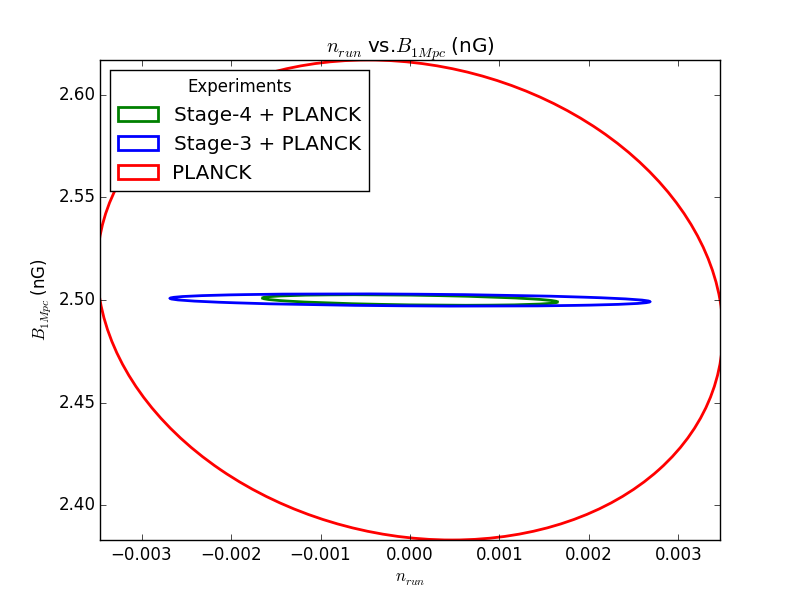
\includegraphics[scale=0.85]{images/contours/nrun.png}
\caption{This is a plot of the 1$\sigma$ confidence contours for $n_{run}$ vs. $B_{1Mpc}$. The red line shows the confidence contour for previous PLANCK data. The blue contour shows the confidence contour for stage-3 CMB experiments plus PLANCK data. The green contour shows the confidence contour for stage-4 CMB experiments plus PLANCK data. The plot shows a large forecasted improvement on the stage-3 and stage-4 precisions on $B_{1Mpc}$ over the previous PLANCK constraints. Improvements on $n_{run}$ increase from PLANCK to stage-3 and again from stage-3 to stage-4.}
\label{fig:nrun}
\end{figure}

\begin{figure}[h]
\centering
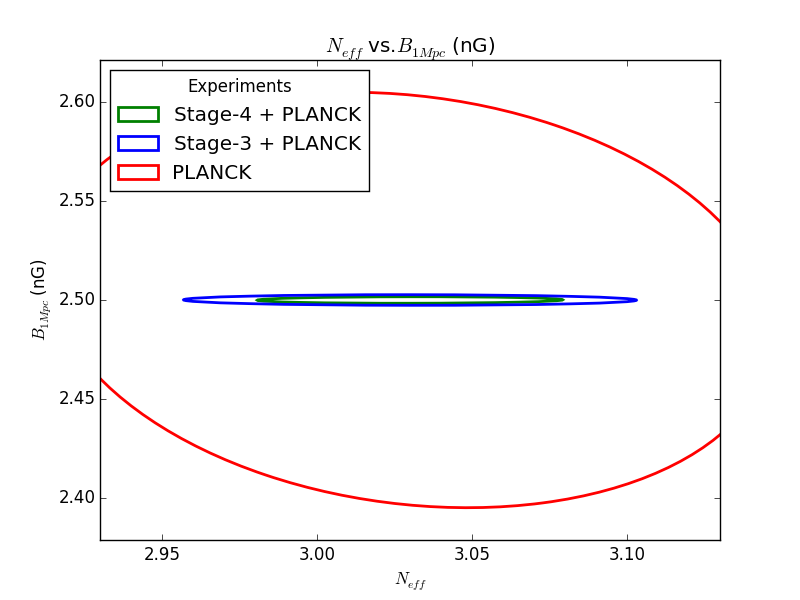
\includegraphics[scale=0.85]{images/contours/neff.png}
\caption{This is a plot of the 1$\sigma$ confidence contours for $N_{eff}$ vs. $B_{1Mpc}$. The red line shows the confidence contour for previous PLANCK data. The blue contour shows the confidence contour for stage-3 CMB experiments plus PLANCK data. The green contour shows the confidence contour for stage-4 CMB experiments plus PLANCK data. The plot shows moderate improvements on $\sigma(B_{1Mpc})$, with stage-4 experiments possessing the tightest constraints, as expected. $N_{eff}$ sees a large forecasted improvement on its constraints from previous PLANCK data. }
\label{fig:neff}
\end{figure}

\begin{figure}[h]
\centering
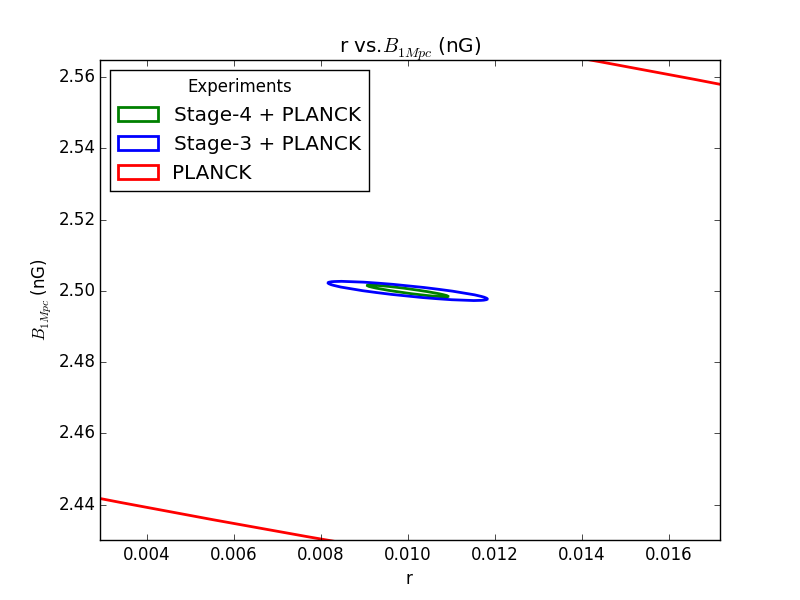
\includegraphics[scale=0.85]{images/contours/52.png}
\caption{This is a plot of the 1$\sigma$ contours for $r$ vs. $B_{1Mpc}$. The red line shows the confidence contour for previous PLANCK data. The blue contour shows the confidence contour for stage-3 CMB experiments plus PLANCK data. The green contour shows the confidence contour for stage-4 CMB experiments plus PLANCK data. There is a large forecasted improvement in both the constraints on $B_{1Mpc}$ and $r$ over previous PLANCK data, however neither stage-3 or stage-4 are expected to break the degeneracy between $B_{1Mpc}$ and $r$.}
\label{fig:r}
\end{figure}

As shown in figure ~\ref{fig:nrun}, stage-3 and stage-4 experiments make major improvements on $B_{1Mpc}$ and moderate improvements over $n_{run}$ from PLANCK results. The gains in precision in $n_{run}$ are significant from stage-3 to stage-4 in contrast to the gains in $B_{1Mpc}$. This relationship between $\sigma({B_{1Mpc})$ and $\sigma({n_{run})$ indicates that future CMB experiments will be effective for providing constraints on $n_{run}$. Additionally, There is a very weak degeneracy between the two parameters according to the PLANCK contour which seems to be broken by the contours from stage-3 and stage-4.

Figure ~\ref{fig:neff} shows that stage-3 and stage-4 experiments make moderate improvements on constraining $N_{eff}$ from current PLANCK results. The graph also shows that within PLANCK data there exists a degeneracy between the $B_{1Mpc}$ and the effective number of neutrinos. Stage-3 and stage-4 appear to break this degeneracy. Given the magnitude of the decrease in the size of the contours from PLANCK to stage-3 to stage-4, there is something to gain from using data from future CMB experiments to constrain $N_{eff}$.

Finally, figure ~\ref{fig:r} shows a drastic improvement on the constraints of $r$ from PLANCK to the next generations. This is to be expected since detecting primordial gravity waves from inflation is one of the primary science goals of ground-based CMB polarisation experiments. Data from stage-3 and stage-4 do not break the degeneracy that existed in PLANCK between $B_{1Mpc}$ and $r$ however. As a result, other methods for constraining the values of these parameters will be needed.
